\chapter{Descripción de la realización}
El equipo del proyecto está formado por el director del proyecto y dos desarrolladores de software; en la figura \ref{fig:organigrama} se puede observar el organigrama del proyecto. El director del proyecto es a su vez el cliente de la solución que se va a desarrollar, por lo que es el que se encargará de validar cada componente principal de la solución; una vez que ha sido correctamente depurado. Los desarrolladores son los encargados del diseño, programación, despliegue, pruebas y documentación del proyecto; la terminación de sus tareas reside en la decisión del director del proyecto una vez que ha comprobado que cumple los requisitos acordados.

\begin{figure}[H]
	\begin{center}
		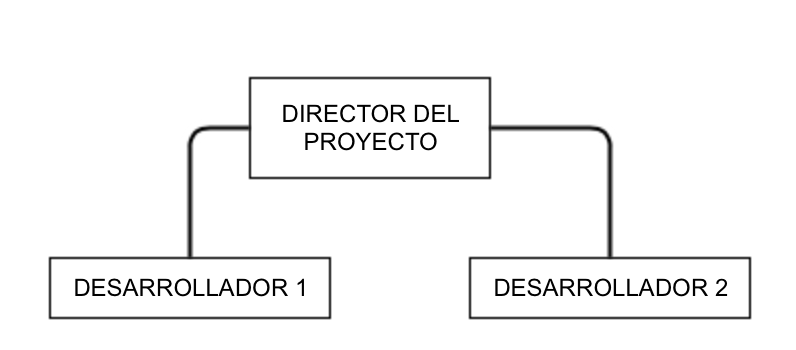
\includegraphics[scale=0.5]{organigrama}
		\caption{Organigrama del proyecto}
		\label{fig:organigrama}
	\end{center}
\end{figure}

La planificación del proyecto se ha desarrollado para poder mantener un ritmo continuo de desarrollo de tipo ágil, y conseguir un aprovechamiento máximo del proyecto. Durante el desarrollo de este proyecto se ha realizado paralelamente pequeños proyectos, por lo que es  necesario que se puedan observar los resultados del desarrollo de la forma más inmediata posible. Para ello, se realizan pequeños prototipos de una funcionalidad que más adelante son integradas en el proyecto. 

La estrategia seguida durante el proyecto puede observarse en la figura 1. Inicialmente se reúnen el director del proyecto con los desarrolladores para reunir los requisitos necesarios y se realiza un diseño de las funcionalidades a incluir, se producen varias iteraciones hasta que todos los requisitos son satisfechos. Una vez finalizado el diseño se pasa al desarrollo, el cual incluye depuración y pruebas unitarias; el desarrollo es parte de los desarrolladores, pero la validación debe ser realizada por el director del proyecto cuando se hayan implementado todos los requisitos de la iteración en ejecución. 

Cuando la iteración del desarrollo ha finalizado correctamente, se pueden añadir nuevos requisitos o pasar a pruebas en calle si han sido programadas con anterioridad con el director del proyecto; algunas pruebas requieren de adaptar parte del programa al carácter de las pruebas. 

La planificación y ejecución de las pruebas deben ser supervisadas por el director del proyecto, y ejecutadas por los desarrolladores. Una vez finalizadas las pruebas, si se han descubierto fallos en el software, se debe realizar una depuración del mismo y si se decide que se requiere ampliar la plataforma se vuelve a iniciar el ciclo.

Las fases del proyecto se puede dividir en los siguientes bloques:
\begin{itemize}
	\item Recolección de requisitos del sistema y estudio de la tecnología necesaria.
	
	\item Desarrollo de la Nube de conductores.
	
	\item Desarrollo de la aplicación para ciclistas.
	
	\item Desarrollo de la \gls{rsu}, \gls{obu} y \gls{hmi}.
	
	\item Verificación del sistema en la calle.
	
	\item Estudio de los resultados y generar documentación.
\end{itemize}

Los hitos del proyecto son las distintas pruebas que se han hecho de funcionalidades
diferentes del sistema. Durante estas pruebas se analiza el rendimiento que se obtiene
de la comunicación del sistema, se proponen y añaden mejoras que serán incluidas en
siguientes pruebas.
\section{Condiciones de ejecución}
Los recursos están definidos en el apartado de ''Presupuestos''. El lugar de trabajo será el departamento de transporte de DeustoTech; en la universidad de Deusto. El horario y calendario son los correspondientes a los lugares de trabajo y según su contrato laboral. Todos los medios materiales, servicios necesarios e instalaciones son provistos por DeustoTech.

DeustoTech es responsable de los servicios provistos: repositorios para el almacenamiento del código, máquinas virtuales y el correcto funcionamiento de todos los sistemas informáticos empleados en sus oficinas. Los programadores a su vez, deben emplear los repositorios de código y copias de seguridad para garantizar la seguridad e integridad del proyecto.

Los desarrolladores y el jefe de proyecto se comunicarán directamente entre ellos; a través del correo electrónico o presencialmente. Aunque todos los requisitos y decisiones deben quedar formalizadas en reunión y reflejadas en el sistema de gestión de actividades empleado en el departamento: Trello. Los cambios en algún requisito o la inclusión de una nueva funcionalidad debe realizarse al finalizar una iteración en ejecución y antes de comenzar otra; es decir, no se parará la implementación de una función si esta ha comenzado su desarrollo, aunque se pueden planear nuevos requisitos para futuras iteraciones. 

El proceso para realizar una modificación, o alguna actividad que impliquen cambios en las especificaciones, diseños o desarrollos realizados, serán presentados para valoración al equipo del proyecto. En caso de aceptación se harán las modificaciones pertinentes en el presupuesto y el plan de trabajo.

La aprobación de cada producto lo dará el cliente (el director del proyecto) en base a las especificaciones que se han acordado en las reuniones durante las fases de requisitos. La validación del proyecto se realizará cuando se hayan completado todos los componentes de la solución final, comprobando que se han cumplido tanto los requisitos como los objetivos que han sido planificados. Tras la prueba final de la plataforma, el director del proyecto decidirá cómo documentar la memoria final, además de los artículos o trabajos derivados que puedan realizarse tras la finalización del presente proyecto.

